\chapter{Literature Review}
\section{Motion Tracking Applications}

Motion tracking, the process of capturing and analyzing the movements of objects or individuals, has become a cornerstone technology in various domains. The integration of advanced sensor systems and artificial intelligence (AI) has significantly enhanced its precision and applicability. Below is an overview of its key applications:

\begin{figure}[h!]
\begin{center}
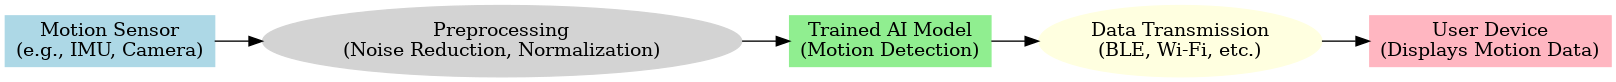
\includegraphics[width=14cm,height=2cm]{images/chapter_2/Motion_Detection_Process_General.png}
\caption{Motion Detection Process General}
\label{fig:enter-label}
\end{center}
\end{figure}

\begin{itemize}
    \item \textbf{Healthcare}
    
    Motion tracking technologies play a pivotal role in healthcare, particularly in physical rehabilitation and movement disorder diagnostics \cite{article:motion_tracking_using_AI}. Systems equipped with motion tracking capabilities allow healthcare professionals to monitor and evaluate patients' movements, ensuring rehabilitation exercises are performed with precision. Gait analysis, a specialized application, aids in diagnosing conditions such as Parkinson’s disease or cerebral palsy, enabling tailored therapeutic interventions. Additionally, fall detection systems, leveraging real-time motion tracking, provide critical support in elder care, mitigating risks associated with sudden falls.

    Example: Wearable devices equipped with accelerometers and gyroscopes track gait patterns in patients with Parkinson’s disease, enabling early detection of irregularities and tailored interventions.

    Benefits: Enhances patient care, promotes early diagnosis, and provides data-driven insights for medical professionals.

    \item \textbf{Sports and Fitness}
    
    In sports, motion tracking enhances performance monitoring and injury prevention. Athletes and coaches use motion analysis to optimize biomechanics, such as joint angles, posture, and movement efficiency. Wearable sensors and AI-based systems enable real-time feedback during training, helping athletes refine their techniques while reducing the likelihood of overuse injuries. Devices like smartwatches and fitness trackers analyze metrics such as stride length, cadence, and heart rate variability. Moreover, motion tracking facilitates data-driven approaches to performance improvement, fostering a competitive edge.
    
    Example: Professional athletes use wearable motion trackers to refine their techniques and assess the biomechanics of their movements during training.
    
    Advances: Real-time feedback mechanisms help coaches and athletes make instant adjustments, maximizing performance.

    \item \textbf{Gaming and Virtual/Augmented Reality (VR/AR)}
    
    The gaming industry and immersive technologies like VR and AR heavily rely on motion tracking to provide intuitive and engaging user experiences. Full-body motion tracking systems, including motion controllers and VR suits, allow users to interact seamlessly with virtual environments. In AR, motion tracking aligns virtual objects with real-world movements, enabling applications in education, entertainment, and remote collaboration. These innovations contribute to the growing demand for lifelike and interactive digital experiences.
    
    Example: Motion controllers in gaming consoles like the PlayStation VR track hand and body movements to provide realistic gameplay experiences.
    
    Impact: Facilitates more natural user interactions and expands applications to virtual training and simulations.

    \item \textbf{Robotics and Automation}
    
    Robotics applications depend on motion tracking for navigation, task execution, and human-robot interaction. Robots equipped with motion tracking systems can perform complex tasks, such as autonomous navigation in dynamic environments or collaborative operations in industrial settings. For example, motion tracking enables precise path planning and obstacle avoidance, critical for autonomous delivery robots and robotic arms used in manufacturing.
    
    Example: Robotic arms in manufacturing use motion tracking to precisely perform repetitive tasks like assembly and packaging.
    
    Benefits: Boosts efficiency, accuracy, and safety in industrial applications.

    \item \textbf{Emerging Applications}
    
    Beyond traditional domains, motion tracking is gaining traction in areas such as filmmaking, where it underpins motion capture (mocap) technology to create lifelike animations. In biomechanics, motion tracking supports research on human movement and ergonomics. Smart home systems utilize gesture-based motion tracking for intuitive control of devices, exemplifying its potential in consumer technologies.
\end{itemize}

\textbf{Role of AI in Motion Tracking}

Artificial intelligence has become indispensable in advancing motion tracking systems. By processing data from inertial measurement units (IMUs) \cite{article:motion_tracking_IMU_upper_limb}, cameras \cite{article:motion_tracking_using_vision}, or other sensors, AI models enable accurate classification and prediction of movements. For instance, AI algorithms can distinguish between activities such as walking, running, or jumping using sensor data from wearable devices. The integration of AI not only enhances the precision of motion tracking but also democratizes its applications by automating complex analyses, thereby broadening accessibility across diverse user groups.


\newpage

% \begin{table}[htb]
% \centering
% \caption{caption here}
% \label{tab:tab_1}
% \begin{tabular}{lll}
% \toprule
% \multicolumn{1}{c}{\textbf{Application Domain}} & \multicolumn{1}{c}{\textbf{Examples}}   & \multicolumn{1}{c}{\textbf{Key Benefits}}         \\
% \hline
% \hline
% Healthcare                                      & Gait analysis, fall detection           & Accurate monitoring, personalized treatment plans \\
% \hline
% Sports                                          & Performance analysis, injury prevention & Optimized training, reduced risk of injuries      \\
% \hline
% Gaming/VR/AR                                    & Immersive experiences                   & Enhanced user interaction, lifelike simulations   \\
% \hline
% Robotics                                        & Path planning, human-robot interaction  & Autonomous navigation, precise task execution    \\
% \hline
% \end{tabular}
% \end{table}

\begin{table}[htb]
\centering
\caption{Applications of Motion Tracking Across Domains}
\label{tab:tab_1}
\begin{tabular}{| >{\centering\arraybackslash}m{3.5cm} | >{\centering\arraybackslash}m{4.5cm} | >{\centering\arraybackslash}m{5cm} |}
\toprule
\textbf{Application Domain}& \textbf{Examples} & \textbf{Key Benefits} \\
\midrule
Healthcare & Gait analysis, fall detection & Accurate monitoring, personalized treatment plans \\
\hline
Sports & Performance tracking, injury prevention & Optimized training, reduced injury risks \\
\hline
Gaming/VR/AR & Immersive VR/AR experiences & Enhanced user interaction, lifelike simulations \\
\hline
Robotics & Path planning, human-robot interaction & Autonomous navigation, precise task execution \\
\bottomrule
\end{tabular}
\end{table}

\section{AI Model Generation Techniques}
The development of AI models for motion tracking involves several stages, from data collection to deployment. These models leverage sensor data, such as accelerometer and gyroscope readings, to detect, classify, and predict movements. Moreover, the generation of AI models for motion tracking involves various methodologies designed to extract meaningful patterns from raw sensor data. These techniques are tailored to meet the specific requirements of motion tracking applications, balancing accuracy, computational efficiency, and scalability. The following sections discuss the key techniques, tools, and frameworks for AI model generation in motion tracking applications.

\begin{figure}[h!]
\begin{center}
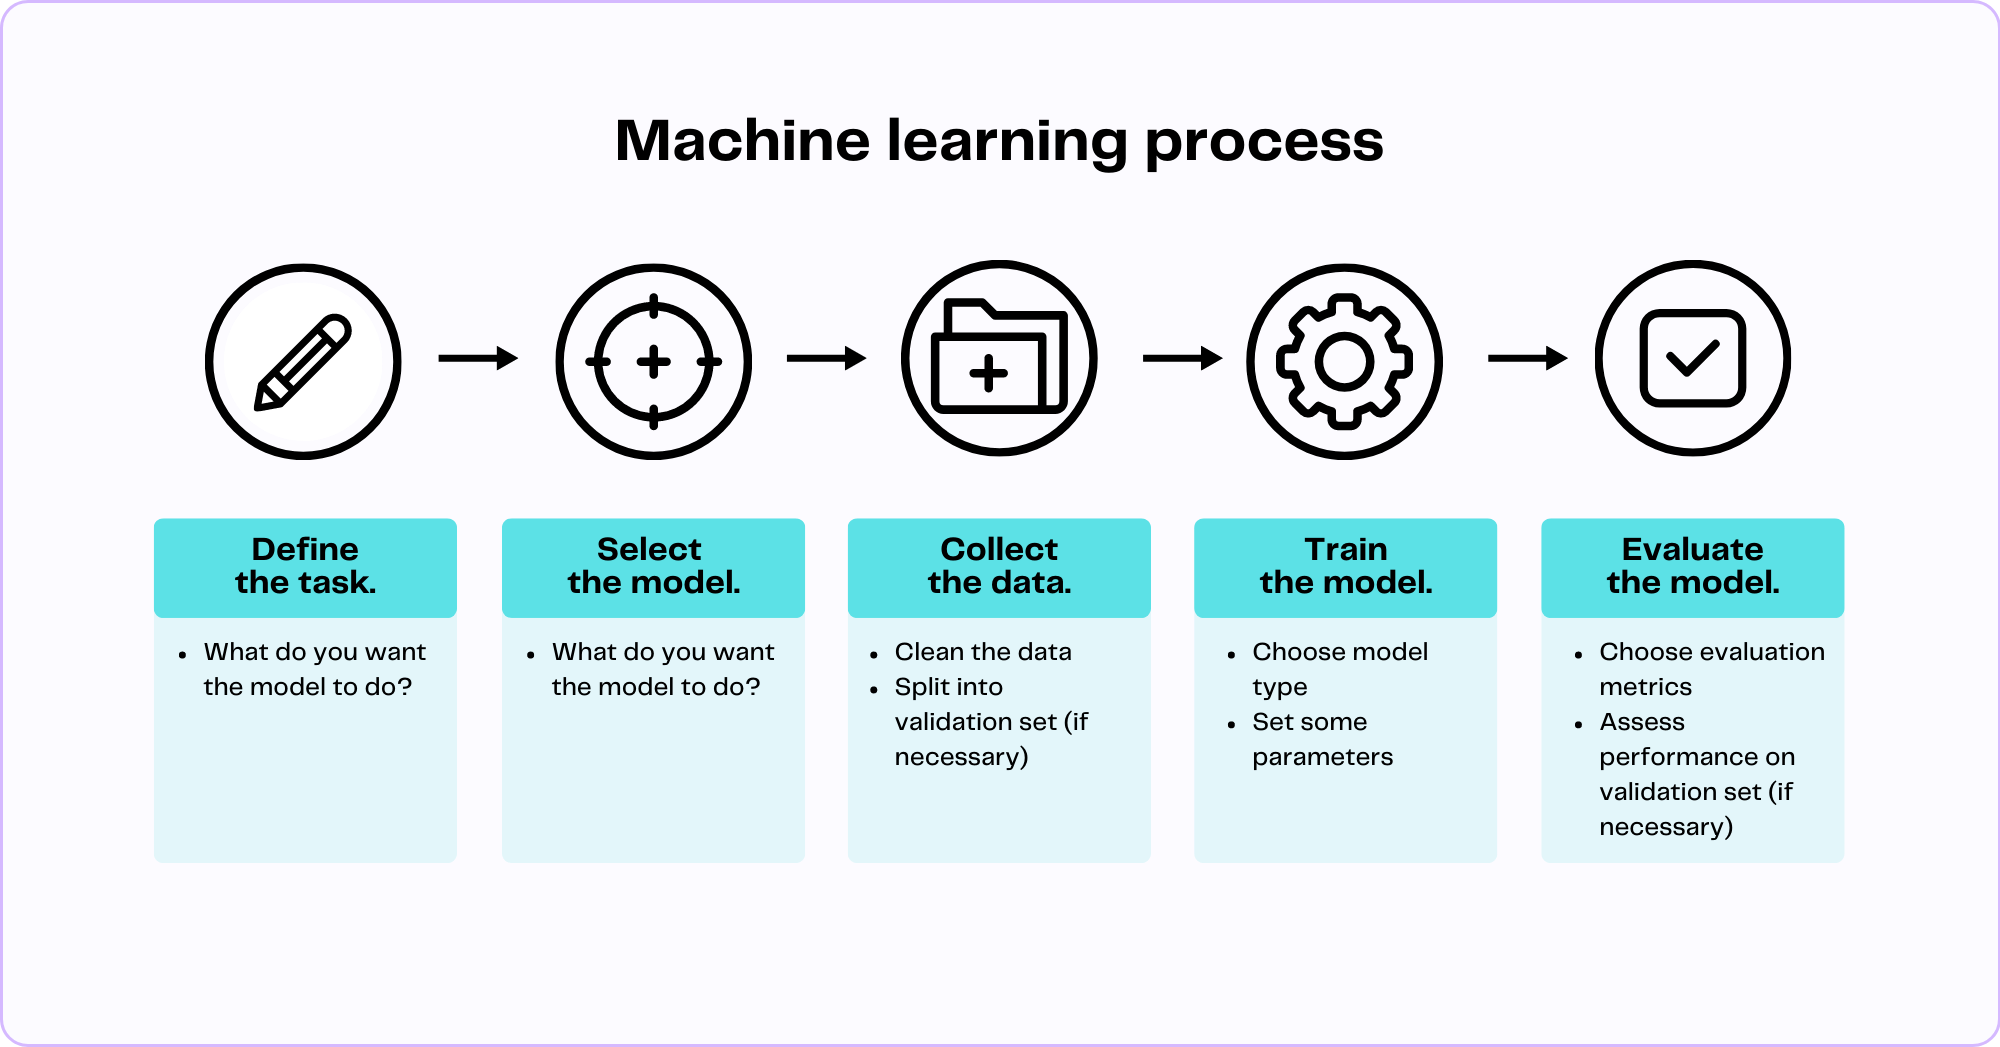
\includegraphics[width=14cm]{images/chapter_2/machine_learning_process.png}
\caption{Machine learning process}
\label{fig:machine_learning_process}
\end{center}
\end{figure}

\subsection{Traditional Machine Learning Approaches}
Traditional machine learning methods rely on extracting handcrafted features from motion data, such as mean, variance, and frequency-domain characteristics. These features are then used to train classifiers, such as Support Vector Machines (SVMs), Decision Trees, and k-Nearest Neighbors (kNN). While effective for specific applications, these methods often require significant domain expertise to design feature extraction pipelines and may struggle to generalize across diverse datasets.

\subsection{Deep Learning Approaches}
Deep learning has revolutionized motion tracking by automating feature extraction and achieving higher accuracy in complex tasks. Neural network architectures such as:

\begin{itemize}
    \item Convolutional Neural Networks (CNNs): Often used for processing spatially structured data like images or time-series motion data.
    \item Recurrent Neural Networks (RNNs) and Long Short-Term Memory Networks (LSTMs): Well-suited for handling sequential data, capturing temporal dependencies in motion signals.
    \item Transformer Models: Emerging as powerful tools for sequence modeling, with applications in activity recognition.
\end{itemize}
Deep learning models can directly process raw sensor data, eliminating the need for manual feature engineering. However, they often require large labeled datasets and computational resources, posing challenges for deployment on resource-constrained devices.

\subsection{Hybrid Approaches}
Hybrid techniques combine the strengths of traditional and deep learning approaches. For instance, traditional feature extraction methods may be integrated with neural networks to enhance model interpretability and efficiency. Such approaches are particularly useful when datasets are small or when computational resources are limited.

\subsection{Tools and Frameworks for Model Generation}
Several tools and frameworks facilitate the development of AI models for motion tracking. These include both general-purpose machine learning libraries and specialized tools designed for edge and real-time applications:

\begin{table}[htb]
\centering
\caption{AI Model Generation Techniques}
\label{tab:tab_2}
\begin{tabular}{ |>{\centering\arraybackslash}m{3.5cm}|>{\centering\arraybackslash}m{5cm}|>{\centering\arraybackslash}m{5cm}| } 
\toprule
\textbf{Framework} &	\textbf{Key Features} &	\textbf{Best Suited For} \\
\midrule
Edge Impulse &	AutoML, TinyML optimization &	Resource-constrained devices \\
\hline
Google MediaPipe &	Real-time tracking, multimodal pipelines &	VR/AR and interactive applications \\
\hline
TensorFlow/PyTorch &	Extensive libraries, flexibility &	Custom AI model development \\
\bottomrule
\end{tabular}
\end{table}

\begin{itemize}
    \item \textbf{Edge Impulse} \cite{web:Edge_Impulse}: A platform designed specifically for edge AI development. Edge Impulse allows developers to collect sensor data, preprocess it, and train lightweight machine learning models optimized for deployment on microcontrollers and other edge devices. Its integrated pipeline simplifies motion tracking by offering pre-built modules for sensor data ingestion and model training.

    \item \textbf{Google MediaPipe} \cite{web:Google_Mediapipe}: A powerful framework for building perception pipelines. MediaPipe provides state-of-the-art solutions for real-time motion tracking using pre-trained AI models, including hand and body pose estimation. It offers a modular design, enabling developers to integrate motion tracking capabilities into applications with minimal effort. MediaPipe’s optimization for mobile and edge devices makes it highly suitable for real-time motion analysis.

    \item \textbf{Google’s Teachable Machine} \cite{web:Google_TeachableMachine}: A web-based tool that simplifies AI model creation for non-experts by providing a no-code interface for training classification models. While primarily focused on general classification tasks, it offers potential for motion tracking applications by enabling quick prototyping of sensor-based models.

    \item \textbf{TensorFlow Lite and PyTorch Mobile} \cite{web:TensorFlowLite}: These frameworks provide tools for deploying lightweight AI models on edge devices. They support quantization and other optimizations, enabling real-time inference on resource-constrained hardware.
\end{itemize}

\begin{table}[htb]
\centering
\caption{Tools and Frameworks Evaluation}
\label{tab:tab_3}
\begin{tabular}{| >{\centering\arraybackslash}m{3.5cm} | >{\centering\arraybackslash}m{3cm} | >{\centering\arraybackslash}m{2cm} | >{\centering\arraybackslash}m{2cm} | >{\centering\arraybackslash}m{2cm} |}
\toprule
\textbf{Tool/Framework} & \textbf{Purpose} & \textbf{Ease of Use} & \textbf{Optimized for Edge?} & \textbf{Real-Time Capabilities} \\
\midrule
Edge Impulse & Sensor-based model development & High & Yes & Moderate \\
\hline
Google MediaPipe & Perception pipelines for motion & Moderate & Yes & High \\
\hline
TensorFlow Lite & Model deployment on edge devices & Moderate & Yes & Moderate \\
\bottomrule
\end{tabular}
\end{table}

\subsection{Data Requirements and Preprocessing}

AI model generation heavily relies on high-quality datasets. In motion tracking, this involves capturing data from sensors like accelerometers, gyroscopes, or cameras. Preprocessing steps include:

\begin{itemize}
    \item Noise Reduction: Filtering out artifacts caused by sensor drift or environmental factors.
    \item Normalization: Ensuring consistent scale across data features.
    \item Segmentation and Labeling: Dividing motion signals into meaningful segments for supervised learning.
\end{itemize}

The pre-processing phase is critical for model performance, as poorly processed data can lead to suboptimal results, regardless of the model used.

% \section{Existing Frameworks}
% Provide an overview of any frameworks already developed for AI-driven motion tracking, along with their limitations.
\section{Benefits in Motion Tracking AI Models}

Motion tracking AI models offer benefits across a wide range of domains, leveraging a combination of advanced algorithms and sensor technology to improve accuracy, efficiency, and user experience. Here are some of the key benefits:

\begin{itemize}
\item \textbf{Improved accuracy}: AI models process large volumes of sensor data to detect and classify motion with high accuracy, minimizing errors in applications such as healthcare diagnostics and sports performance analysis.

\item \textbf{Real-time feedback}: Real-time processing enables immediate feedback, which is important for applications such as rehabilitation exercises, sports training, and interactive VR/AR systems.

\item \textbf{Scalability}: AI models can be deployed across multiple platforms, from mobile devices to industrial robots, ensuring adaptability to a wide range of hardware configurations and use cases.

\item \textbf{Personalization}: Machine learning algorithms enable motion tracking systems to be tailored to each user, improving the suitability and effectiveness of applications such as fitness tracking and rehabilitation.

\item \textbf{Cost-effectiveness}: Automating complex tasks reduces the reliance on manual intervention, leading to cost savings in areas such as manufacturing and elder care.

\item \textbf{Wider Accessibility}: Lightweight AI models optimized for edge devices make advanced motion tracking accessible in resource-constrained environments, expanding usage to underserved areas or lower-budget projects.

\item \textbf{Data-Driven Insights}: AI-powered analytics generate actionable insights from motion data, supporting decision-making in sports coaching, healthcare treatment planning, and industrial operations.

\end{itemize}

By integrating these benefits, AI-driven motion tracking continues to transform traditional operations, enabling innovative solutions and empowering users across multiple domains.


\section{Challenges in Motion Tracking AI Models}
Despite significant advancements, the development of AI models for motion tracking faces several challenges. Addressing these obstacles is crucial for achieving robust, scalable, and real-time systems, particularly in resource-constrained environments.

\begin{enumerate}
    \item \textbf{Data Collection and Quality}
        \begin{itemize}
            \item Sensor Noise: Motion tracking heavily relies on data from IMUs, cameras, or other sensors. However, these devices often produce noisy signals due to environmental factors, hardware limitations, or sensor drift.
            \item Dataset Diversity: Capturing diverse datasets that account for variations in users, activities, and environments remains challenging. Models trained on narrow datasets often fail to generalize to unseen scenarios.
            \item Labeling Complexity: Accurate labeling of motion data is time-intensive and often requires domain expertise. Ambiguous or inconsistent labels can degrade model performance.
        \end{itemize}
    
% Diagram Suggestion: A flowchart illustrating the data collection pipeline, highlighting points where noise and inconsistencies can occur, could clarify this process.

    \item \textbf{Computational Constraints}
        \begin{itemize}
            \item Edge Deployment: Many motion tracking applications require AI models to run on edge devices like microcontrollers or smartphones. These devices have limited computational resources, making it difficult to deploy complex models without optimization.
            \item Real-Time Processing: Motion tracking systems often demand low-latency inference for real-time applications such as sports performance monitoring or interactive VR. Balancing model complexity and speed remains a significant challenge.
        \end{itemize}
% Diagram Suggestion: A comparison chart showing computational power, latency, and energy efficiency for various platforms (e.g., cloud vs. edge devices).

    \item \textbf{Generalizability and Adaptability}
        \begin{itemize}
            \item Domain-Specific Customization: AI models for motion tracking must adapt to different use cases, such as healthcare, sports, or gaming. Creating adaptable models without significant retraining is a complex task.
            \item Cross-Device Consistency: Variations in sensor quality and configurations across devices often lead to inconsistencies in data, requiring robust model designs or calibration techniques.
        \end{itemize}
% Table Suggestion: A table comparing domain-specific requirements (e.g., healthcare vs. gaming) and their implications for model design.

    \item \textbf{Data Privacy and Security}
        \begin{itemize}
            \item Sensitive Data: Motion tracking often involves personal data, such as healthcare metrics or identifiable movement patterns. Ensuring data privacy while enabling AI training and inference is a significant concern.
            \item Federated Learning: Emerging techniques like federated learning offer potential solutions by training models locally on devices without sharing raw data. However, these approaches introduce additional complexity and may reduce model performance.
        \end{itemize}

    \item \textbf{Integration Challenges}
        \begin{itemize}
            \item Hardware-Software Compatibility: Motion tracking systems require seamless integration between hardware (e.g., sensors) and software (e.g., AI frameworks). Discrepancies can lead to performance bottlenecks.
            \item Scalability: Scaling solutions across diverse hardware ecosystems and applications is difficult, particularly when designing for global or multi-user scenarios.
        \end{itemize}

\end{enumerate}

\section{Challenges in Motion Tracking and AI Integration}

Despite advancements, several challenges remain in the integration of AI and motion tracking technologies. Addressing these challenges is essential for widespread adoption and innovation.

\begin{enumerate}
    \item \textbf{Hardware Constraints}
        \begin{itemize}
            \item Resource Limitations: Many motion tracking applications rely on low-power devices with limited processing and storage capabilities.
            \item Impact: AI models need to be optimized for efficient inference on edge devices without compromising accuracy or be trade-offs between model accuracy and computational efficiency.
            \item Example: Difficulty in running deep learning models on microcontrollers due to memory constraints.
        \end{itemize}

    \item \textbf{Data Quality and Variability}
        \begin{itemize}
            \item Challenges: Sensor data can be noisy, inconsistent, or affected by environmental factors such as temperature, humidity, or interference.
            \item Impact: Requires robust preprocessing techniques and models capable of handling variability.
            \item Example: Wearables giving inaccurate step counts due to motion artifacts.
        \end{itemize}

    \item \textbf{Scalability of AI Models}
        \begin{itemize}
            \item Issue: Training large-scale AI models for motion tracking requires extensive computational resources and large datasets.
            \item Impact: Limits the ability of small organizations or individual researchers to develop and deploy advanced systems.
            \item Solution: Use of pre-trained models and transfer learning.
        \end{itemize}

    \item \textbf{Latency in Real-Time Applications}
        \begin{itemize}
            \item Problem: Real-time applications like gaming, VR/AR, and robotics demand low-latency processing, which is challenging for computationally intensive AI models.
            \item Impact: Can lead to lag or poor user experience.
            \item Solution: Development of lightweight, optimized AI models using quantization or pruning.
        \end{itemize}

    \item \textbf{Ethical and Privacy Concerns}
        \begin{itemize}
            \item Concern: Collecting and processing motion data raises questions about user privacy and data security.
            \item Impact: Limits user adoption and raises regulatory challenges.
            \item Solution: Adoption of privacy-preserving techniques like federated learning and on-device processing.
        \end{itemize}
\end{enumerate}

%%%%%%%%%%%%%%%%%%

% \section{Federated Learning and Privacy-Preserving AI}
% To address privacy concerns, federated learning techniques are being explored for motion tracking applications.

% Description: Data is processed locally on the device, and only model updates are shared with central servers.
% Impact: Maintains user privacy while enabling continuous model improvement.
% % Visual Suggestion: A schematic diagram illustrating federated learning in the context of wearable motion tracking.

% \subsection{Multimodal Sensor Fusion}
% Combining data from multiple sensors (e.g., IMUs, cameras, LiDAR) enhances motion tracking accuracy and robustness. AI models can learn to fuse these inputs effectively.

% Example: Autonomous vehicles using multimodal inputs for navigation.
% Advances: AI architectures designed to process multimodal data streams in real time.
% % Visual Suggestion: A layered diagram showing how data from different sensors is fused and processed by AI models.

% \section{Justification for Your Approach}
% Discuss why you believe AI-based frameworks could be a solution and the potential advantages over traditional methods.

\section{Current Trends in Motion Tracking and AI Integration}
In recent years, motion tracking has evolved significantly due to advancements in AI and sensor technology. Emerging trends highlight how these technologies are converging to deliver innovative solutions across various domains.

\subsection{Wearable Motion Tracking Systems}
Wearable devices equipped with IMUs, GPS, and other sensors have become mainstream in sports, healthcare, and consumer electronics. These systems leverage AI for real-time analysis and provide actionable insights.

\begin{itemize}
    \item Advances in Wearables: AI has made these systems smarter by providing real-time insights and personalized feedback. Integration of AI models on low-power edge devices, enabling on-device analysis and feedback.
    \item Example: Smart fitness bands like Fitbit and Apple Watch use AI to analyze fall detection in elderly care, step counts, heart rates, and sleep patterns accurately.
    \item Impact: Improved accessibility and affordability of motion tracking systems for consumers.
\end{itemize}
% Visual Suggestion: A timeline showing the evolution of wearable motion tracking devices over the past decade.

\subsection{AI-Driven Real-Time Tracking}
Real-time motion tracking is critical in domains like gaming, VR/AR, and autonomous robotics. AI algorithms now support faster and more accurate motion prediction.

\begin{itemize}
    \item Key Trend: Development of lightweight AI models that operate efficiently on edge devices, ensuring low latency in processing.
    \item Example: Google MediaPipe’s real-time hand tracking achieves high accuracy with minimal computational requirements.
    \item Applications: Immersive VR/AR systems, autonomous robotics, and interactive gaming experiences.
\end{itemize}
    
% Visual Suggestion: A bar graph comparing the inference speeds of AI models optimized for real-time tracking.

\subsection{Multimodal Sensor Fusion}
Combining data from multiple sensors improves the robustness and accuracy of motion tracking systems. AI plays a crucial role in fusing data streams from IMUs, cameras, and LiDAR sensors.
\begin{itemize}
    \item Example: Autonomous vehicles use multimodal sensor fusion for precise navigation in dynamic environments.
    \item Benefits: Enhanced motion prediction, reduced errors, and improved adaptability to environmental changes.
\end{itemize}

\subsection{Edge AI and Federated Learning}
The rise of edge computing has transformed how motion tracking data is processed.
\begin{itemize}
    \item Edge AI: AI models are deployed on devices rather than relying on cloud infrastructure, reducing latency and improving privacy.
    
    Example: Smart glasses with embedded AI for gesture recognition.
    
    \item Federated Learning: A privacy-preserving technique where AI models are trained locally on devices, and only model updates are shared with central servers.
    
    Example: Smartphones using federated learning for activity recognition without sharing raw motion data.
\end{itemize}

\subsection{Emerging Domains and Applications}
AI-driven motion tracking is extending into less conventional areas, creating novel opportunities:
\begin{itemize}
    \item Smart Cities: Monitoring pedestrian and traffic movements to optimize urban planning.
    \item Healthcare Innovations: Using motion data for predictive health diagnostics.
    \item Cinematic Applications: AI-assisted motion capture for creating realistic animations in films and video games.
\end{itemize}

    % "Trend": [
    %     "Wearable and Portable Systems",
    %     "Real-Time Motion Tracking Using AI",
    %     "Multimodal Sensor Fusion",
    %     "Edge AI and Federated Learning",
    %     "Emerging Domains and Applications"
    % ],
    % "Applications": [
    %     "Health monitoring, sports analysis",
    %     "VR/AR, gaming, robotics",
    %     "Autonomous vehicles, industrial robotics",
    %     "Gesture recognition, privacy-preserving applications",
    %     "Smart cities, healthcare innovations, cinematic motion capture"
    % ],
    % "AI Impact": [
    %     "Real-time insights, personalized feedback",
    %     "Low latency, efficient processing",
    %     "Improved accuracy, robustness",
    %     "Enhanced privacy, reduced cloud dependence",
    %     "New opportunities, predictive analytics"
    % ]